\documentclass{article}
\usepackage{amsmath}
\usepackage{amssymb}
\usepackage{amsthm}
\usepackage{listings}
\usepackage{float}
\usepackage{graphicx}
\usepackage[includefoot,bottom=12pt]{geometry}
\usepackage{hyperref}
\usepackage{subcaption}
\usepackage{fancyhdr}
\usepackage{bbm}
\usepackage{tikz}

\definecolor{codegray}{rgb}{0.5,0.5,0.5}
\definecolor{codeblue}{rgb}{0.25,0.5,0.75}
\definecolor{codegreen}{rgb}{0,0.6,0}
\definecolor{codered}{rgb}{0.75,0.25,0.25}

\lstdefinestyle{mystyle}{
    backgroundcolor=\color{white},   
    commentstyle=\color{codegreen},
    keywordstyle=\color{codeblue},
    numberstyle=\tiny\color{codegray},
    stringstyle=\color{codered},
    basicstyle=\ttfamily\footnotesize,
    breakatwhitespace=false,         
    breaklines=true,                 
    captionpos=b,                    
    keepspaces=true,                 
    numbers=left,                    
    numbersep=5pt,                  
    showspaces=false,                
    showstringspaces=false,
    showtabs=false,                  
    tabsize=4
}

\lstset{style=mystyle}


\geometry{left=1.25in}

\pagestyle{fancy}
% \fancyhead{}
% \fancyfoot{}

\makeatletter
\newcommand*{\centernot}{%
  \mathpalette\@centernot
}
\def\@centernot#1#2{%
  \mathrel{%
    \rlap{%
      \settowidth\dimen@{$\m@th#1{#2}$}%
      \kern.5\dimen@
      \settowidth\dimen@{$\m@th#1=$}%
      \kern-.5\dimen@
      $\m@th#1\not$%
    }%
    {#2}%
  }%
}
\makeatother

\newcommand{\independent}{\perp\mkern-9.5mu\perp}
\newcommand{\notindependent}{\centernot{\independent}}

\fancyhead[R]{23B0940, 23B1081, 23B1045}
\fancyhead[L]{\leftmark}

\renewcommand{\sectionmark}[1]{\markboth{#1}{}}

\title{AML Assignment-1}

\author{Aditya Neeraje, Niral Charan, Rishi Kalra}

\date{\today}

\begin{document}

\maketitle
\tableofcontents

\pagenumbering{gobble}

\newpage

\pagenumbering{arabic}
\section{Generating and Triangulating the Graph}
Some of the preprocessing starts when we initialize the Inference class itself. We create an instance of the Graph class, and add edges in it according to the cliques in the given graph. We also note how many cliques each vertex is part of, which comes in handy later to speed up finding simplicial vertices.\\
Here, to avoid incorrect counting of the number of cliques a node is in if one of the input cliques is a subset of another, I sort the cliques in increasing order of sizes, and consider a clique only if it is maximal (and consider only one clique if there are multiple instances of the exact same clique in the graph).\\
We then store the graph's state (adjacency list, number of cliques and number of neighbours, etc\.) so that we can revert to the original state after triangulating using one heuristic (say, min-neighbours), before triangulating based on another heuristic (say, min-fill).\\
\\
Then, when \texttt{triangulate\_and\_get\_cliques} is called, the heuristic is used to find a close-to-optimal triangulation of the graph. Since the implementation of all heuristics is fundamentally very similar, I will here only elaborate on the implementation of min-neighbours. First, we separate the corner case of nodes with no neighbours, and start maintaining a list of simplicial nodes. While there are nodes yet to be included in the ordering, we search for simplicial nodes and add them to the ordering, and implicity delete it from the graph by setting its number of neighbours to 0 (which is the check I use later to see if a node is deleted). We keep updating the cliques by removing nodes which have been eliminated, until we no longer find any simplicial vertex. Now, we choose the vertex with the fewest neighbours, and create a new clique with it and its neighbours. We also delete all those cliques which earlier contained this vertex. Now, if the addition of this clique causes a previous clique to not remain maximal, we delete that clique. We keep repeating this process until all nodes are eliminated.
The two heuristics I have implemented are min-fill and min-neighbours, which were found to be quite effective strategies in \url{https://cse.unl.edu/~choueiry/Documents/Kjaerulff-TR-1990.pdf}. I choose the better of the two returned graphs based on the maximum clique size I would get using them. Note that I have not implemented min-weight since all vertices have equal \lq\lq weight\rq\rq\ since every variable is binary, and hence this would be equivalent to min-neighbours.
\section{Junction Tree Creation}
Now, I pass the variable elimination order to the JunctionTree class' init function. For each node being eliminated, I create the clique corresponding to the same. Non-maximal cliques are identified and deleted using the following lines of code:
\begin{lstlisting}[language=Python]
  for j in range(len(self.cliques)-1):
  sep_set = clique & self.cliques[j]
  self.sep_sets[-1].append(-len(sep_set))
  if len(sep_set)==len(clique):
      self.cliques.pop()
      self.sep_sets.pop()
      break
\end{lstlisting}

After this, I call \texttt{get\_junction\_tree()} on the same, which runs Kruskal's algorithm to get the MST given all the cliques, with edge weights being the size of the intersection of two cliques. Our implementation also allows for edges of weight 0.\\
The \texttt{get\_junction\_tree()} internally calls a function that creates a parent relationship between nodes, which is useful later because, for better complexity, we have implemented the Junction Tree algorithm as comprising of one upward pass and one downward pass.\\
\section{Upward Pass}
While there is a node with no children and with a defined parent (it is not the root of its connected component), we identify the sep\_set connecting it and its parent, and call the marginalization function over its potential so as to compute the message to be sent. This message is multiplied into the potentials of the parent. Here, an important difference in implementation from \url{https://ocw.mit.edu/courses/6-438-algorithms-for-inference-fall-2014/1faaccb44f78c4f4e99c6814842082a0_MIT6_438F14_Lec8.pdf} needs to be mentioned - we are not treating the distributions as positive, and the multiplication operation as being invertible. However, we note that if two separate children send a message of 0 to a parent, during the downward pass, factoring out the message of 0 sent by one child does not change the fact that the potential will remain as 0, thus maintaining a memory of whether a message has been multiplied by 0 at least two times, works.\\
With this in mind, we have the following code snippet which makes our inverse-multiplication step work:
\begin{lstlisting}[language=Python]
  def product_func(a, b):
  if b!=0:
      return a[0]*b, a[1]*b
  elif a[0]==0:
      return 0, 0
  else:
      return 0, a[0]

def product_inv_func(a, b):
  if b!=0:
      return a[0]//b, a[1]//b
  return a[1], a[1]
\end{lstlisting}
Our goal with this \texttt{product\_inv\_func} is to emulate what is done in the MIT slides:
\begin{figure}[H]
  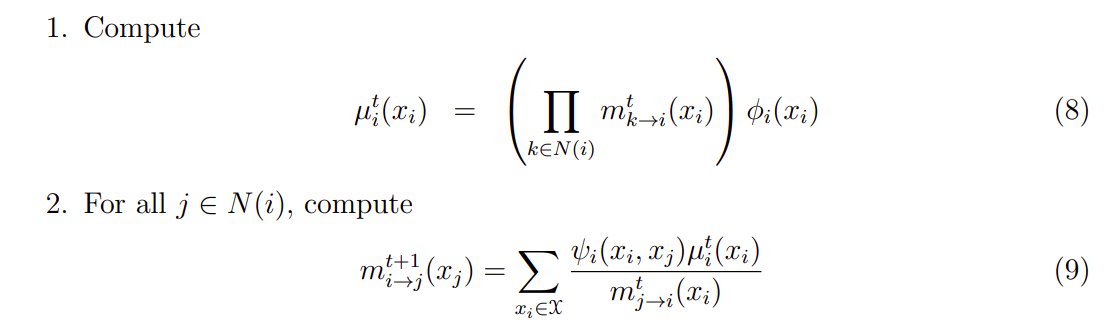
\includegraphics[width=0.7\textwidth]{Slides_Eq89.png}
\end{figure}
\section{Downward Pass}
After sending messages upward to the root, note that we can immediately get answers to two queries - Z and top k most probable assignments, without needing a downward pass. This is exactly how we have implemented it in the code, wherein we read off Z first, and then carry out a downward pass. For the most probable assignments, we needed a separate composition and marginalization function, so that part is done independently of the Z and marginal queries.\\
Now, to explain how the Downward Pass works in the case of the marginal probabilities query, we simply reverse the order in which messages are sent during the upward pass. From the parent of the current node, we first \lq\lq factor out \rq\rq\ the message sent to the parent by the child. For this, the \texttt{product\_inv\_func} defined above is useful, to deal with the case of some messages being 0.\\
Then, from the parent we send a message downward, computed by marginalizing the parent's potentials over the sep-set.  
\begin{lstlisting}[language=Python]
  def downward_pass(self, marginalization_func):
  self.upward_pass_order.reverse()
  for curr_node in self.upward_pass_order:
      parent = self.parents[curr_node]
      sep_set = self.cliques[curr_node].variables&self.cliques[parent].variables
      self.cliques[parent].factor_out(sep_set, self.cliques[curr_node].message)
      message = self.cliques[parent].marginalize(sep_set, marginalization_func)
      self.cliques[curr_node].factor_in(sep_set, message)
      self.cliques[parent].factor_in(sep_set, self.cliques[curr_node].message)
\end{lstlisting}
Note that self.cliques[curr\_node].message need not be updated since we never do anything with the message after the downward pass, even though technically if a message were sent again it would be different from the original message.
\section{Marginal Probability Queries}
We have already seen \texttt{upward\_pass} and \texttt{downward\_pass}. Using \texttt{upward\_pass} alone, we get at the root node a set of potentials which has factored in messages from all other nodes as well. Marginalizing these potentials over an empty set of variables gives us the required value of Z.\\
Then, we call the downward pass. After that, for every variable, we identify one clique in which it is present, and marginalize this clique's potential with respect to that variable, and divide by Z to get the marginal probability of that variable.\\
\begin{lstlisting}[language=Python]
  self.junction_tree.downward_pass(sum_func)
  marginals = []
  for var in range(self.variables_count):
      for clique in self.junction_tree.cliques:
          if var in clique.variables:
              marginals.append([value/self.Z for value in clique.marginalize({var}, sum_func)])
              break
  for clique in self.junction_tree.cliques:
      clique.restore_state()
  return marginals
\end{lstlisting}
In the code above, \texttt{sum\_func} is simply addition (but defined over 2-tuples).
\section{MAP Assignment}
The Maximum A Posteriori assignment is the assignment which is most probable with respect to the probability distribution over assignments. Here, given that Z is fixed, it is simply the assignment which has the highest product of induced clique potentials. Just like marginals can be computed using the Sum-Product method, MAP queries can be answered using the Max-Product method, where Max is the marginalization function and Product is the combination function (here, I am borrowing terminology from Exercise 9.19 of Koller Friedman)
\begin{figure}[H]
  \centering
  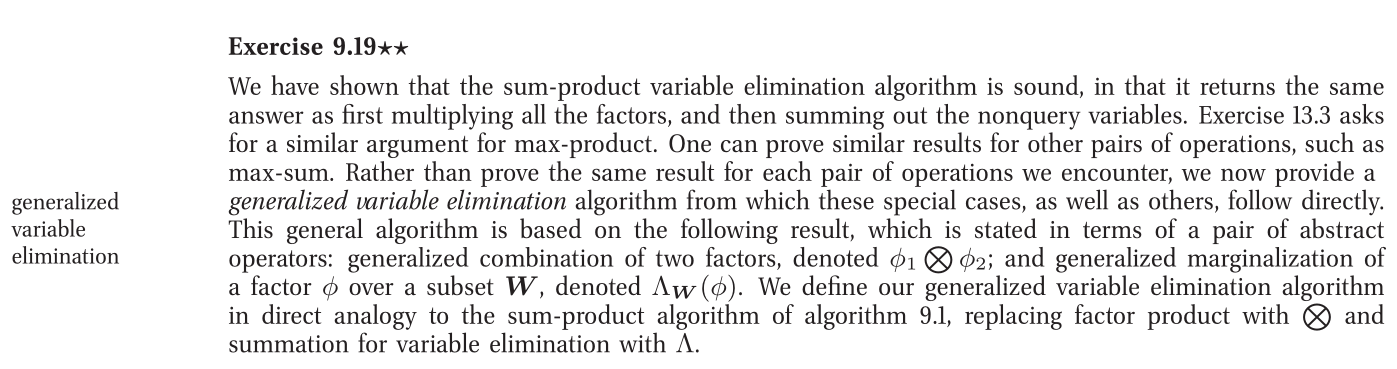
\includegraphics[width=0.9\textwidth]{Ex9.19-KF.png}
\end{figure} 
\textbf{Note: }There is a slight difference between my definition of the marginalization function and the book's definition, but that is solely for ease of coding it up. My marginalization function takes two elements at a time and sums them up, whereas the book's definition takes a list of potentials to be marginalized and returns one value for each such list. Since the operators being used are commutative and associative, there is no practical difference between the two definitions.\\
The combination part is the same as in the Sum-Product algorithm, but when we have to marginalize over a subset of variables, for every assignment to that subset we choose the assignment to all other variables that maximizes the product of potentials seen so far.\\
As noted in Exercise 9.19 and the course slides, this is amenable to variable elimination. Since VE elimination is equivalent to one-directional message passing over a junction tree, MAP queries can be handled by junction trees too. While \lq\lq factoring in\rq\rq\ a message, we multiply the current potentials by the corresponding potentials of the message, and during marginalization we take the maximum over all potentials corresponding to a particular assignment to a subclique.\\
This is in fact a special case of the k-most probable assignments query, and hence I move on to explain the k-most probable queries implementation.
\section{Top k assignments}
I am using the \texttt{heapq} module to maintain, for each partial assignment which we encounter during the message passing algorithm, the (at most k) top assignments that are consistent with that partial assignment. Note that this is also a special case of Exercise 9.19. I thus include here my implementation of the marginalization and combination functions:
\begin{lstlisting}[language=Python]
  def marginalization_for_k_map_assignments(a, b):
  ### NOTE that b is completely deleted after this. This is only useful when there is no backward pass needed, as in our case
  while b:
      heapq.heappush(a, heapq.heappop(b))
  while len(a) > k: 
      heapq.heappop(a)
  return a
  
def composition_for_k_map_assignments(a, b): # a and b are both heapq's
  result = []
  b_list = list(b)
  while a:
      a_top = heapq.heappop(a)
      for b_element in b_list:
          heapq.heappush(result, (a_top[0]*b_element[0], "".join([a_top[1][i] if a_top[1][i]!='x' else b_element[1][i] for i in range(len(a_top[1]))])))
  while len(result) > k:
      heapq.heappop(result)
  return result
\end{lstlisting}
To explain the above code, note that the marginalization function is called during upward passes, when, given two \texttt{heapq}'s with up to k assignments each, we want to reduce it to one \texttt{heapq} with up to k assignments. This final \texttt{heapq} contains the k most probable extensions of a given partial assignment.\\
In a similar vein, the combination step involves taking the k largest products corresponding to a partial assignment in an incoming message, the k largest products corresponding to that partial assignment in the existing potential table, and selecting the best k (or fewer) potentials from amongst all their products.\\
The most probable assignment is, of course, the MAP assignment, and hence these functions, with k=1, can be used to find the MAP assignment.
I am storing the partial assignment observed so far with a string consisting of '0', '1' and 'x' to denote 0, 1 and undecided.
\section{References}
\begin{itemize}
  \item \url{https://ocw.mit.edu/courses/6-438-algorithms-for-inference-fall-2014/1faaccb44f78c4f4e99c6814842082a0_MIT6_438F14_Lec8.pdf}
  \item \url{https://cse.unl.edu/~choueiry/Documents/Kjaerulff-TR-1990.pdf}
  \item Koller and Friedman, Probabilistic Graphical Models
\end{itemize}
\section{Contributions}
\begin{itemize}
  \item Code - Aditya Neeraje
  \item Report - Aditya Neeraje, Rishi Kalra
  \item Generating Testcases and Brute Force code for testing - Aditya Neeraje
  \item Identifying a research paper on different triangulation methods - Niral Charan
\end{itemize}
\end{document}